%% abtex2-modelo-trabalho-academico.tex, v-1.9.6 laurocesar
%% Copyright 2012-2016 by abnTeX2 group at http://www.abntex.net.br/ 
%%
%% This work may be distributed and/or modified under the
%% conditions of the LaTeX Project Public License, either version 1.3
%% of this license or (at your option) any later version.
%% The latest version of this license is in
%%   http://www.latex-project.org/lppl.txt
%% and version 1.3 or later is part of all distributions of LaTeX
%% version 2005/12/01 or later.
%%
%% This work has the LPPL maintenance status `maintained'.
%% 
%% The Current Maintainer of this work is the abnTeX2 team, led
%% by Lauro César Araujo. Further information are available on 
%% http://www.abntex.net.br/
%%
%% This work consists of the files abntex2-modelo-trabalho-academico.tex,
%% abntex2-modelo-include-comandos and abntex2-modelo-references.bib
%%

% ------------------------------------------------------------------------
% ------------------------------------------------------------------------
% abnTeX2: Modelo de Trabalho Academico (tese de doutorado, dissertacao de
% mestrado e trabalhos monograficos em geral) em conformidade com 
% ABNT NBR 14724:2011: Informacao e documentacao - Trabalhos academicos -
% Apresentacao
% ------------------------------------------------------------------------
% ------------------------------------------------------------------------

\documentclass[
	% -- opções da classe memoir --
	12pt,				% tamanho da fonte
	openright,			% capítulos começam em pág ímpar (insere página vazia caso preciso)
	oneside,			% para impressão em recto e verso. Oposto a oneside
	a4paper,			% tamanho do papel. 
	% -- opções da classe abntex2 --
	%chapter=TITLE,		% títulos de capítulos convertidos em letras maiúsculas
	%section=TITLE,		% títulos de seções convertidos em letras maiúsculas
	%subsection=TITLE,	% títulos de subseções convertidos em letras maiúsculas
	%subsubsection=TITLE,% títulos de subsubseções convertidos em letras maiúsculas
	% -- opções do pacote babel --
	english,			% idioma adicional para hifenização
	%french,				% idioma adicional para hifenização
	%spanish,			% idioma adicional para hifenização
	brazil				% o último idioma é o principal do documento
	]{abntex2}

% ---
% Pacotes básicos 
% ---
\usepackage{lmodern}			% Usa a fonte Latin Modern			
\usepackage[T1]{fontenc}		% Selecao de codigos de fonte.
\usepackage[utf8]{inputenc}		% Codificacao do documento (conversão automática dos acentos)
\usepackage{lastpage}			% Usado pela Ficha catalográfica
\usepackage{indentfirst}		% Indenta o primeiro parágrafo de cada seção.
\usepackage{color}				% Controle das cores
\usepackage{graphicx}			% Inclusão de gráficos
\usepackage{microtype} 			% para melhorias de justificação
\usepackage{subfig}
\usepackage{float}
\usepackage{listofsymbols}

%\usepackage{reledmac}


%pacote da tabela
\usepackage{multirow}
% ---
%	
% ---
% Pacotes adicionais, usados apenas no âmbito do Modelo Canônico do abnteX2
% ---
\usepackage{lipsum}				% para geração de dummy text
% ---

% ---
% Pacotes de citações
% ---
\usepackage[brazilian,hyperpageref]{backref}	 % Paginas com as citações na bibl
%\usepackage[alf]{abntex2cite}	% Citações padrão ABNT
\usepackage[alf,abnt-etal-list=0,abnt-etal-cite=3]{abntex2cite}
 
% --- 
% CONFIGURAÇÕES DE PACOTES
% --- 

% ---
% Configurações do pacote backref
% Usado sem a opção hyperpageref de backref
\renewcommand{\backrefpagesname}{Citado na(s) página(s):~}
% Texto padrão antes do número das páginas
\renewcommand{\backref}{}
% Define os textos da citação
\renewcommand*{\backrefalt}[4]{
	\ifcase #1 %
		Nenhuma citação no texto.%
	\or
		Citado na página #2.%
	\else
		Citado #1 vezes nas páginas #2.%
	\fi}%
% ---

% ---
% Informações de dados para CAPA e FOLHA DE ROSTO
% ---
\titulo{Sistema de Aquisição e Transmissão de Dados Usando Sensor de Flexão Bioinspirado}
\autor{Wederson Medeiros Silva}
\local{Belém -- Pará}
\data{2018}
\orientador{Prof. Dr. Roberto Menezes Rodriguez}
\coorientador{Prof. Dr. João Crisóstomo Weyl A. Costa}
\instituicao{
  Universidade Federal do Pará -- UFPa
  \par
  Instituto de Tecnologia -- ITEC
  \par
  Faculdade de Engenharia da Computação e Telecomunicações -- FCT}
\tipotrabalho{Trabalho de Conclusão de Curso}

% O preambulo deve conter o tipo do trabalho, o objetivo, 
% o nome da instituição e a área de concentração 
\preambulo{Trabalho de Conclusão de Curso apresentado para obtenção do
título de Bacharel em Engenharia da Computação. Instituto de Tecnologia. Faculdade de Engenharia da Computação e Telecomunicações. Universidade Federal do Pará.
}
% ---


% ---
% Configurações de aparência do PDF final

% alterando o aspecto da cor azul
\definecolor{blue}{RGB}{41,5,195}

% informações do PDF
\makeatletter
\hypersetup{
     	%pagebackref=true,
		pdftitle={\@title}, 
		pdfauthor={\@author},
    	pdfsubject={\imprimirpreambulo},
	    pdfcreator={LaTeX with abnTeX2},
		pdfkeywords={abnt}{latex}{abntex}{abntex2}{trabalho acadêmico}, 
		colorlinks=true,       		% false: boxed links; true: colored links
    	linkcolor=black,          	% color of internal links
    	citecolor=black,        		% color of links to bibliography
    	filecolor=black,      		% color of file links
		urlcolor=black,
		bookmarksdepth=4
}
\makeatother
% --- 

% --- 
% Espaçamentos entre linhas e parágrafos 
% --- 

% O tamanho do parágrafo é dado por:
\setlength{\parindent}{1.3cm}

% Controle do espaçamento entre um parágrafo e outro:
\setlength{\parskip}{0.2cm}  % tente também \onelineskip

% ---
% compila o indice
% ---
\makeindex
% ---

% ----
% Início do documento
% ----
\begin{document}

% Seleciona o idioma do documento (conforme pacotes do babel)
%\selectlanguage{english}
\selectlanguage{brazil}

% Retira espaço extra obsoleto entre as frases.
\frenchspacing 

% ----------------------------------------------------------
% ELEMENTOS PRÉ-TEXTUAIS
% ----------------------------------------------------------
% \pretextual

% ---
% Capa
% ---
\renewcommand{\imprimircapa}{
\begin{capa}

\center

\includegraphics[scale=0.4]{figures/ufpa_logo.jpg}

 { \ABNTEXchapterfont 
 UNIVERSIDADE FEDERAL DO PARÁ\\
 INSTITUTO DE TECNOLOGIA\\
 FACULDADE DE ENGENHARIA ELÉTRICA E BIOMÉDICA\\}
   \vspace*{4.0cm}
 
 { \ABNTEXchapterfont\large
   \textbf{\imprimirautor}}
   \vspace*{3.0cm}

 {\ABNTEXchapterfont\LARGE
 \textbf{\imprimirtitulo}}

 \vspace*{\fill}
 {\large\imprimirlocal}
 \par
 {\large\imprimirdata}
 \vspace*{1cm}
\end{capa}
}
% ---
% Capa
% ---
\imprimircapa
% ---

% ---
% Folha de rosto
% (o * indica que haverá a ficha bibliográfica)
% ---
%%Folha de Rosto
\makeatletter
\renewcommand{\folhaderostocontent}{
  \begin{center}

    \vspace*{0.08cm}
    {\ABNTEXchapterfont\Large
     \imprimirautor}

    \vspace*{\fill}\vspace*{\fill}
    {\ABNTEXchapterfont\LARGE
     \textbf{\imprimirtitulo}}
     \vspace*{\fill}

    \abntex@ifnotempty{\imprimirpreambulo}{
      \hspace{.45\textwidth}
      \begin{minipage}{.5\textwidth}
         \imprimirpreambulo\\    
      \end{minipage}%
       \vspace*{\fill}
    }%
    
    {\ABNTEXchapterfont\Large
     \imprimirorientadorRotulo
     \ABNTEXsectionfont~\imprimirorientador\par}
    
    {\ABNTEXchapterfont\Large
     \imprimircoorientadorRotulo
     \ABNTEXsectionfont~\imprimircoorientador}%

    \vspace*{\fill}
    {\large\imprimirlocal}
    \par
    {\large\imprimirdata}
  \end{center}
}
\makeatother

% ---
% Folha de rosto
% (o * indica que haverá a ficha bibliográfica)
% ---
\imprimirfolhaderosto*
% ---
% ---
% Inserir a ficha bibliografica
% ---

% Isto é um exemplo de Ficha Catalográfica, ou ``Dados internacionais de
% catalogação-na-publicação''. Você pode utilizar este modelo como referência. 
% Porém, provavelmente a biblioteca da sua universidade lhe fornecerá um PDF
% com a ficha catalográfica definitiva após a defesa do trabalho. Quando estiver
% com o documento, salve-o como PDF no diretório do seu projeto e substitua todo
% o conteúdo de implementação deste arquivo pelo comando abaixo:
%
% \begin{fichacatalografica}
%     \includepdf{fig_ficha_catalografica.pdf}
% \end{fichacatalografica}

\begin{fichacatalografica}
	\sffamily
	\vspace*{\fill}					% Posição vertical
	\begin{center}					% Minipage Centralizado
	\fbox{\begin{minipage}[c][8cm]{13.5cm}		% Largura
	\small
	\imprimirautor
	%Sobrenome, Nome do autor
	
	\hspace{0.5cm} \imprimirtitulo  / \imprimirautor. --
	\imprimirlocal, \imprimirdata-
	
	\hspace{0.5cm} \pageref{LastPage} p. : il. (algumas color.) ; 30 cm.\\
	
	\hspace{0.5cm} \imprimirorientadorRotulo~\imprimirorientador\\
	
	\hspace{0.5cm} \imprimircoorientadorRotulo~\imprimircoorientador\\
	
	\hspace{0.5cm}
	\parbox[t]{\textwidth}{\imprimirtipotrabalho~--~\imprimirinstituicao,
	\imprimirdata.}\\
	
	\hspace{0.5cm}
		1. Modo fantasma de segunda camada.
		2. Taxa agregada.
		3. \textit{Vectoring}.
		4. EVM.
		I. \imprimirorientador.
		II. Universidade Federal do Pará.
		III. Faculdade de Engenharia Elétrica e Biomédica.
		IV. \imprimirtitulo\\ 		
	\end{minipage}}
	\end{center}
\end{fichacatalografica}
% ---
% ---

% ---
% Inserir folha de aprovação
% ---

% Isto é um exemplo de Folha de aprovação, elemento obrigatório da NBR
% 14724/2011 (seção 4.2.1.3). Você pode utilizar este modelo até a aprovação
% do trabalho. Após isso, substitua todo o conteúdo deste arquivo por uma
% imagem da página assinada pela banca com o comando abaixo:
%
% \includepdf{folhadeaprovacao_final.pdf}
%
\begin{folhadeaprovacao}

  \begin{center}
    {\ABNTEXchapterfont\large\imprimirautor}

    \vspace*{\fill}\vspace*{\fill}
    \begin{center}
      \ABNTEXchapterfont\bfseries\Large\imprimirtitulo
    \end{center}
    \vspace*{\fill}
    
    \hspace{.45\textwidth}
    \begin{minipage}{.5\textwidth}
        \imprimirpreambulo
    \end{minipage}%
    \vspace*{\fill}
   \end{center}
        
   Trabalho aprovado. \imprimirlocal, 24 de dezembro de 2018:

   Conceito: .
   
   \assinatura{\textbf{\imprimirorientador} \\ Orientador} 
   \assinatura{\textbf{\imprimircoorientador} \\ Coorientador}
   \assinatura{\textbf{Prof. Dr. Gilvan Borges} \\ Convidado 1}
  % \assinatura{\textbf{Prof. Dr. Somebody else} \\ Convidado 2}
   %\assinatura{\textbf{Professor} \\ Convidado 3}
      
   \begin{center}
    \vspace*{0.5cm}
    {\large\imprimirlocal}
    \par
    {\large\imprimirdata}
    \vspace*{1cm}
  \end{center}
  
\end{folhadeaprovacao}
% ---

% ---
% Dedicatória
% ---
\begin{dedicatoria}
   \vspace*{\fill}
   \centering
   \noindent
   \textit{ Este trabalho é dedicado...} \vspace*{\fill}
\end{dedicatoria}
% ---

% ---
% Agradecimentos
% ---
\begin{agradecimentos}
Agradeço ao Professor Dr. ...
\end{agradecimentos}
% ---
% ---

% ---
% Epígrafe
% ---
\begin{epigrafe}
    \vspace*{\fill}
	\begin{flushright}
		\textit{``Não vos amoldeis às estruturas deste mundo, ...)}
	\end{flushright}
\end{epigrafe}
% ---

% ---
% RESUMOS
% ---

% resumo em português
\setlength{\absparsep}{18pt} % ajusta o espaçamento dos parágrafos do resumo
\begin{resumo}
%\setlength{\parindent}{1.5cm}
%\indent
%\hangindent=3.7cm
\hspace{1.5cm}O modo \textit{fronthaul} de redes 5G ...
	
 \textbf{Palavras-chaves}: Modo fantasma. 
\end{resumo}

% resumo em inglês
\begin{resumo}[Abstract]
 \begin{otherlanguage*}{english}
\hspace{1.5cm}Phantom mode has...

   \vspace{\onelineskip}
 
   \noindent 
   \textbf{Keywords}: Phantom mode. 
 \end{otherlanguage*}
\end{resumo}


% ---
% inserir lista de ilustrações
% ---
\pdfbookmark[0]{\listfigurename}{lof}
\listoffigures*
\cleardoublepage
% ---

% ---
% inserir lista de tabelas
% ---
\pdfbookmark[0]{\listtablename}{lot}
\listoftables*
\cleardoublepage
% ---

% ---
% inserir lista de abreviaturas e siglas
% ---
%\imprimirlistadesiglas
\begin{siglas}
 \item[AWG]\textit{American Wire Gauge}
 \item[AXT]\textit{Alien crosstalk} 
 \item[BBU]\textit{Baseband Unit}
 \item[CAGR]\textit{Compound Annual Growth Rate}
 \item[CM]Conversão de modo
 \item[CST]\textit{Computer Simulation Technology}
 \item[DMT]\textit{Discrete Multitone}
 \item[DSL]\textit{Digital Subscriber Line}
 \item[EVM]\textit{Error Vector Magnitude}
 \item[FEXT]\textit{Far-End Crosstalk}
 \item[FT]Função de transferência
 \item[FTTH]\textit{Fiber-to-the-Home}
 \item[IoT]\textit{Internet of Things}
 \item[ITU]\textit{International Telecommunication Union}
 \item[MD]Modo diferencial
 \item[MF1]Modo fantasma de 1ª camada 
 \item[MF2]Modo fantasma de 2ª camada
 \item[MIMO]\textit{Multiple-Input Multiple-Output}
 \item[NEXT]\textit{Near-End Crosstalk}
 \item[RSIR]\textit{Signal-to-Noise Ratio}
 \item[SP]Modo \textit{split-pair}
 \item[STP]\textit{Shielded Twisted Pair}
 \item[UTP]\textit{Unshielded Twisted Pair}
 \item[VNA]\textit{Vector Network Analyzer}
 \item[WS]Modo \textit{wire-shield}
\end{siglas}
% ---

% ---
% inserir lista de símbolos
% ---
\begin{simbolos}
  \item[$\alpha$] Contante de atenuação
  \item[$\beta$] Contante de fase
  \item[$\gamma$] Contante de propagação
  \item[$\Gamma_{L}$] Coeficiente de reflexão na carga
  \item[$\delta$] Constante da restrição de potência transmissão
  \item[$\Delta_f$ ] Subcanais ou tons em Hz
  \item[$ \Gamma $]  Gap de $RSIR$
  \item[$ \Lambda $] Matriz que contém os elementos da diagonal principal de $\mathbf{H}$
  \item[$\rho$] Máscara espectral utilizada pelo sistema DSL
  %  \item[
  \item[${\sigma}^{2}$]  Densidade espectral de potência potência do ruído Gaussiano branco aditivo
\end{simbolos}
% ---

% ---
% inserir o sumario
% ---
\pdfbookmark[0]{\contentsname}{toc}
\tableofcontents*
\cleardoublepage
% ---



% ----------------------------------------------------------
% GUIA DAYNARA
% ----------------------------------------------------------
%{\color{green}
%1- Introdução 
%
%Seção 1: Contexto:
%
%	-Contexto da tecnologia, contendo um histórico das evoluções ADSL – VDSL – G. Fast 
%	
%	-Apontar limitações dos sistemas em relação a transmissão (taxa agregada)
%	
%	-Quais as soluções que estão sendo investigadas
%	
%	-Uma das soluções é buscar modos de transmissão alternativos
%	
%	-Modo fantasma, split-pair e wire-shield 
%	
%Seção 2: Trabalhos relacionados (até onde eles abordaram)
%
%Seção 3: *Motivação:
%Por que pesquisar esta área e esse tema de modos alternativos de transmissão, onde poderia ser aplicados (5G, XG.), etc.;
%
%Seção 4: *Justificativa:
%Quais são exatamente as contribuições, o que eu fiz a mais em relação ao que já existe.
%
%Seção 6:*Objetivos
%
%Seção 5:*Resumo da metodologia
%
%Seção :*organização do trabalho
%}
%{\color{red}


% ----------------------------------------------------------
% ELEMENTOS TEXTUAIS
% ----------------------------------------------------------
\textual

\chapter{Introdução} % ou \input{arquivoexterno}
		
		Contextualização; Estado da arte (se tiver); Motivação; O que vai fazer; Metodologia; O que terá no resto do documento;


	% --------------------- 
	%	REFERENCIAL TEÓRICO	
	% --------------------- 
	
	\chapter{Referencial Teórico}

		\section{Sensor Flex}
		Sensores de flexão, mais conhecidos como sensores flex, são resistores analógicos que trabalham como divisores de tensão analógicos. Dentro desses sensores existem elementos resistivos de carbono junto a um fino substrato flexível. Mais carbono significa menos resistência. Quando o substrato é torcido o sensor produz uma resistência relativa ao raio da torção. \cite{solanki2013sign}.

	\begin{figure}[!h]
		\centering
		\caption{Sensor de Flexão}
		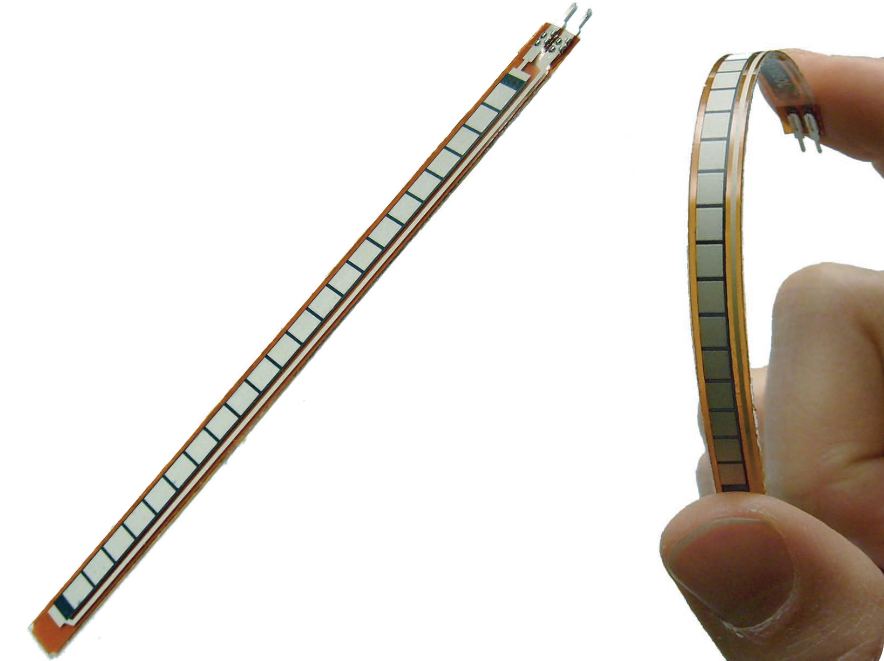
\includegraphics[width=12cm,keepaspectratio=true]{./figures/flex-sensor1.png}
		\fonte{Site Sparkfun}%
		\label{Fig:flex-sensor1}
	\end{figure}

		\section{Potenciômetro}
		O potenciômetro é um componente eletrônico que permite, através do giro do seu eixo, a variação da resistência entre seus terminais. Eles são constituídos por um elemento de resistência, que pode ser de carbono ou fio de nicromo, sobre o qual corre uma lingüeta, denominada cursor. Dentre as características do potenciômetro estão o valor máximo de sua resistência, seu número de voltas, seu grau máximo de giro (aproximado) e se ele é do tipo linear ou logarítmico \cite{ncb2012eletronicabasica}.


		\begin{figure}[h!]
			\centering
  		\caption{Funcionamento do potenciômetro linear}
  		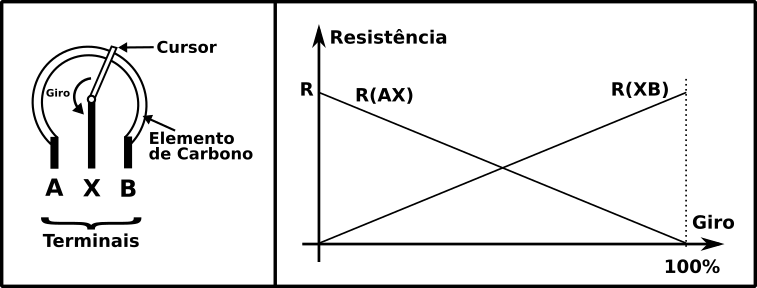
\includegraphics[scale=0.7]{./figures/potentiometer1.png}
			\fonte{Modificado de~\cite{ncb2012eletronicabasica}.}
  		\label{Fig:potentiometer1}
		\end{figure}

		Segundo a lei de Ohm ($V = R.I$), dada uma corrente constante, ao variar a resistência teremos uma variação da tensão. Sendo assim, ao girar o eixo do potenciômetro, dependendo do sentido do giro, perceberemos um aumento ou diminuição da tensão naquele ponto. Partindo de um ponto extremo com resistência mínima até o outro ponto extremo no qual a resistência deverá ser a máxima característica do componente.

		\section{Movimentação dos dedos}
		Na mão, os tendões funcionam como cordas que conectam os músculos do antebraço aos ossos da mão. Nos dedos, os tendões passam por dentro de uma série de polias, que formam uma espécie de túnel. Isso permite manter os tendões próximos aos ossos da mão, aumentando a força nos dedos e diminuindo o gasto de energia. Ao movimentar o dedo, o músculo se contrai para que o tendão deslize por entre as polias. \cite{drricardocirurgiao}
 
		\begin{figure}[h!]
			\centering
  		\caption{Movimento do dedo através do tendão}
  		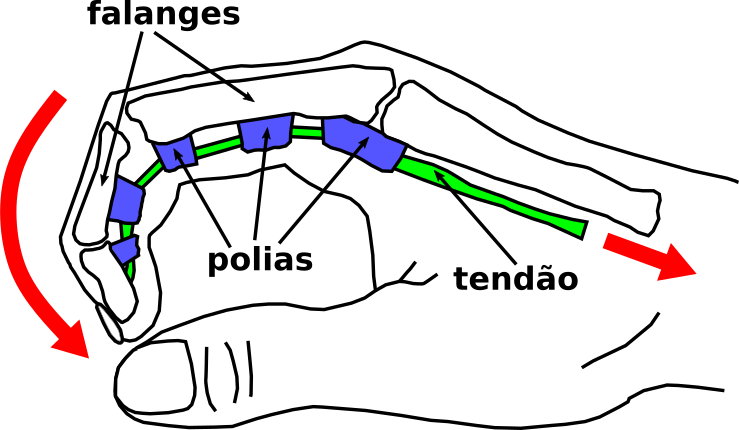
\includegraphics[scale=0.5]{./figures/hand-tendon-flex1.png}
  		\label{Fig:hand-tendon-flex1}
		\end{figure}


		\section{Arduino}
		O Arduino é uma plataforma eletrônica de código aberto (\textit{open-source}) que é baseada em \textit{hardware} e \textit{software} fáceis de usar. As placas Arduino são capazes de ler entradas como o acionamento de um sensor, o pressionamento de um botão, ou uma mensagem do Twitter. E pode transformar essas entradas em saídas como a ativação de um motor, o acendimento de um LED ou até a publicação de algo online. O comportamento dessa placa pode ser programado usando sua interface de desenvolvimento (IDE), que por sua vez, envia as instruções necessárias para o microcontrolador instalado na placa.\cite{arduinosite}
		
		\begin{figure}[h!]
			\centering
			\caption{Placa Arduino modelo Nano \cite{arduinonanosite}}
  		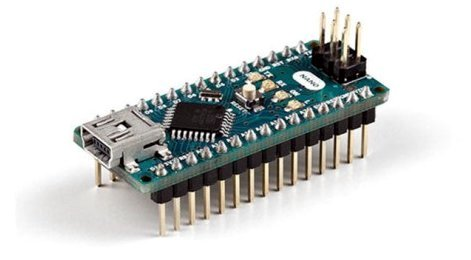
\includegraphics[scale=0.7]{./figures/arduino-nano1.jpg}
  		\label{Fig:arduino-nano1}
		\end{figure}

		\section{Módulo RF 433 Mhz}
		O módulo de rádio frequência 433 Mhz é composto por um par que contém um transmissor e um receptor, ele opera com modulação AM e é uma alternativa para projetos de baixo custo que queiram usar comunicação sem fio entre microcontroladores Arduino ou outros. O par de módulos pode alcançar até 200 metros sem obstáculos, usando antenas e dependendo da tensão aplicada.\cite{institutodigitalrf}


	% ----------------------------
	%	TRABALHO PROPRIAMENTE DITO	
	% ----------------------------
	
	\chapter{Trabalho Propriamente Dito}

		\section{Teoria da coisa}
			Como foi demonstrado na figura \ref{Fig:hand-tendon-flex1}, através dos tendões, passando por polias, têm-se a movimentação dos dedos na mão. Baseado nessa biomecânica de movimento, foi desenvolvido um sistema mecânico semelhante, com o intuito de criar um sensor de flexão de dedos, atrelado a um transmissor de dados.
			
			Inicialmente foi verificado o deslocamento de um fio durante a flexão dos dedos. Para isso, com a mão inicialmente extendida e o dorso voltado para cima, uma das pontas de um fio foi presa na ponta de um dos dedos. O local inicial da outra ponta do fio foi marcada no dorso mão.

			Após a flexão dos dedos o fio se movimentou em uma direção criando um deslocamento (d) do fio em relação ao ponto marcado.

%\begin{figure}[H]
%	\caption{Cabo de pares trançados.}
%	\centering
%	\subfloat[Sem blindagem]{
%		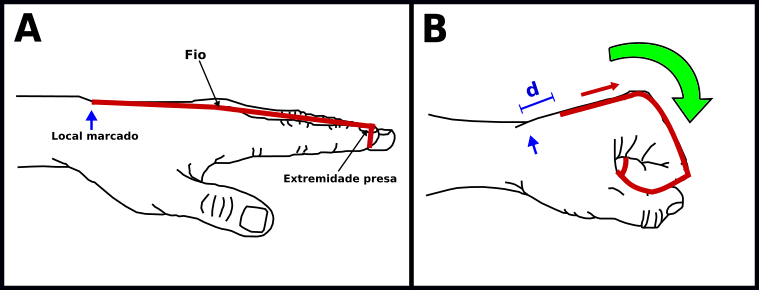
\includegraphics[width=7cm,keepaspectratio=true]{./figures/hand-wire-flex1.png}
%		\label{Fig:UTP}}
 
%	\centering
%	\subfloat[Com blindagem]{
%		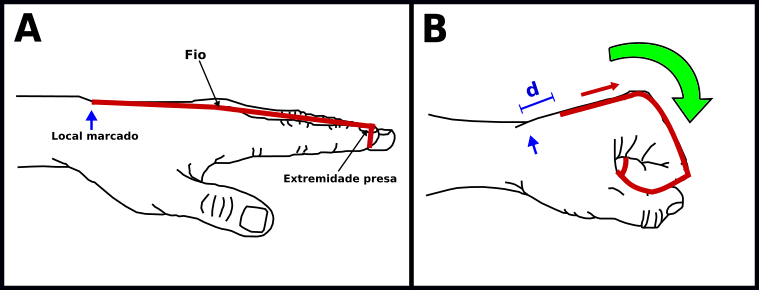
\includegraphics[width=7cm,keepaspectratio=true]{./figures/hand-wire-flex1.png}
%		\label{Fig:STP}}
%	\fonte{.}%
%	\label{Fig:Par}
%\end{figure}

\begin{figure}[!htb]
   \centering
   \caption{ (a) Mão em posição inicial. (b) Mão após flexão.}
   \subfloat[]
   {
     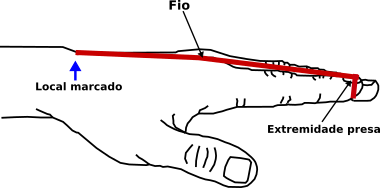
\includegraphics[width=8cm,keepaspectratio=true]{./figures/hand-wire-steady1.png}
   }
   \centering
   \subfloat[]
   { 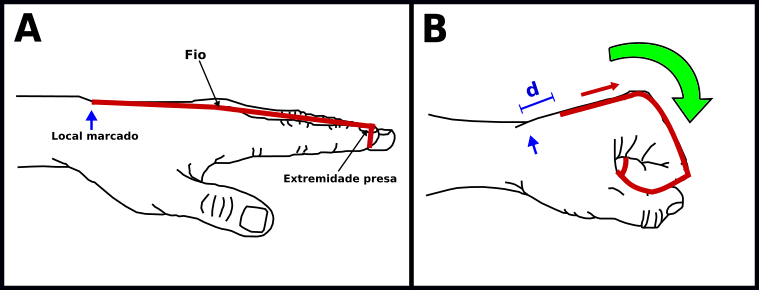
\includegraphics[width=6cm,keepaspectratio=true]{./figures/hand-wire-flex1.png}
   }
   \label{Fig:hand-wire-steady-and-flex}
   \fonte{Produzido pelo autor}
 \end{figure}



			Após examinar esse movimento, foi decidido criar e instalar todo o sistema em uma luva. Fios foram presos às extremidades dos dedos da luva, passando por polias plásticas que servem de guias. Na extremidade oposta, os fios são conectados à pequenos potenciômetros que variam de acordo com o sentido do movimento de cada fio. Sendo assim, para os cinco dedos de cada mão, são utilizados cinco fios e cinco potenciômetros.

			A variação de cada potenciômetro é captada por um microcontrolador que processa esse sinal antes de despachá-lo para o transmissor. O módulo transmissor envia por rádio frequência, mensagens em formato de números inteiros que representam a posição atual de cada dedo.

		\begin{figure}[h!]
			\centering
			\caption{Captação do sinal}
  		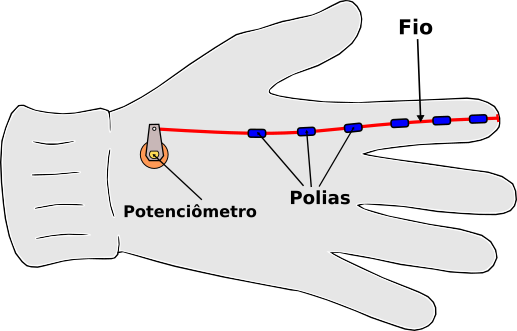
\includegraphics[scale=0.7]{./figures/glove-wire-pot1.png}
  		\label{Fig:glove-and-transmitter1}
			\fonte{Produzido pelo autor}
		\end{figure}

			O módulo receptor de rádio frequência, capta as mensagens e as envia ao microcontrolador conectado. Este por sua vez, processa a mensagem e transmite aos respectivos componentes e atuadores daquela aplicação.

			Para este trabalho, um pequeno carrinho, foi o sistema escolhido para ser controlado pela luva. Para isso, um protocolo de transmissão foi desenvolvido para traduzir os movimentos dos dedos da luva em direções para o carrinho.

	\begin{figure}[!htb]
  	\centering
   	\caption{ (a) Transmissão do sinal. (b) Recepção do sinal.}
   	\subfloat[]
   	{
     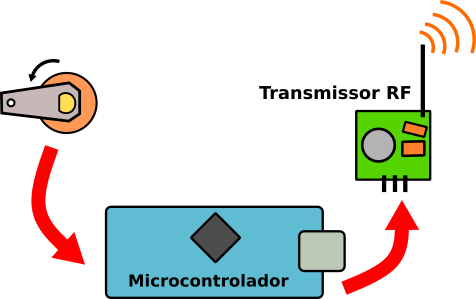
\includegraphics[width=7cm,keepaspectratio=true]{./figures/transmitter-module1.png}
    }
   	\centering
   	\subfloat[]
   	{ 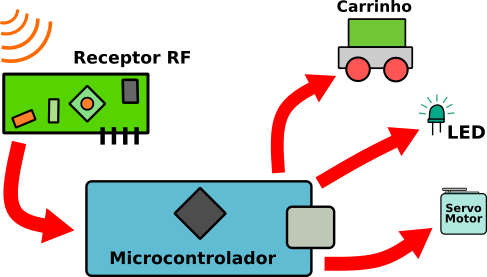
\includegraphics[width=7cm,keepaspectratio=true]{./figures/receptor-module1.png}
   	}
   	\label{Fig:transmitter-and-receptor}
   	\fonte{Produzido pelo autor}
 		\end{figure}


		\section{Medidas e Posicionamento}	

			O sistema de captação e transmissão de sinal que seria embarcado na luva, foi projetado para ser de móvel, leve, alimentado por uma bateria, caber no dorso da mão e ter custo relativamente menor em relação à soluções com sensores flex tradicionais. O sistema dever ser de fácil reprodução e o mais adaptável possível à outras formas de transmissão além da rádio frequência, caso sejam necessárias futuramente.

			\subsection{Componentes}

			O primeiro desafio foi escolher, dentre os componentes disponíveis, quais seriam utilizados para compor a eletrônica presente na placa de circuito impresso que estaria embarcada na luva.

			O potenciômetro foi o primeiro componente a ser definido para o projeto. Isso porque, este seria o componente que estaria em maior número na placa. O modelo escolhido deveria ser pequeno suficiente para manter uma distância adequada para outros potenciômetros e componentes. Seu cursor deveria ser de fácil giro, para que pudesse ser acionado apenas pelo deslocamento do fio. Seu ângulo de giro total precisava ser mínimo, para que o menor grau de giro correspondesse à maior variação possível, facilitando assim a percepção pelo microcontrolador.

			O potenciômetro que mais se aproximou das especificações acima foi retirado de um servo motor modelo MG996R da marca TowerPro. Este servo apresentava problemas de controle e não estava mais sendo usado, porém, seu potenciômetro interno estava funcionando perfeitamente. Este potenciômetro possui dimensão aproximada de 13 $mm$ x 13 $mm$, resistência máxima de $5 k\Omega$, giro aproximado de $200^{o}$ e pouca resistência ao girar seu cursor. 

			Um pequeno pedaço de PVC expandido foi conectado ao cursor do potenciômetro para facilitar o giro e para amarrar uma das extremidades de um fio.

			O microcontrolador escolhido para processar os dados recebidos de cada potenciômetro foi o Arduíno modelo Nano. Isso porque ele é leve, ocupa uma área de apenas 45$mm$ x 17$mm$, possui vasta documentação e disponibilidade no mercado, além de ser compatível com diversos módulos externos e possuir custo menor do que outros modelos da família Arduíno.

			Para transmitir e receber o sinal, foi escolhido para o projeto o par de RF 433$Mhz$, que é leve e de baixo custo comparado à outras soluções de transmissão de dados.

			Finalmente, para alimentar esse aparato eletrônico, foi escolhida uma pequena bateria Li-Po que estava disponível no laboratório. Esta possui 300$mAh$, 7.4$V$ de tensão nominal e ocupa um espaço de 45$mm$ x 12.5$mm$.

			\subsection{Dimensões e Posicionamento}

			Após medições realizadas no dorso da luva vestida que serviu de modelo para o projeto, foi decidido que as dimêncões máximas da placa de circuito impresso (PCI) deveriam ser de aproximadamente 72$mm$ x 58$mm$. Sendo assim, usando o software QCAD, que é gratuito para o sistema Linux, e organizando os compoenntes dentro de suas dimensões aproximadas, chegou-se ao seguinte layout \ref{Fig:size-glove-module1}.

		\begin{figure}[h!]
			\centering
			\caption{Dimensões aproximadas da PCI e seus componentes}
  		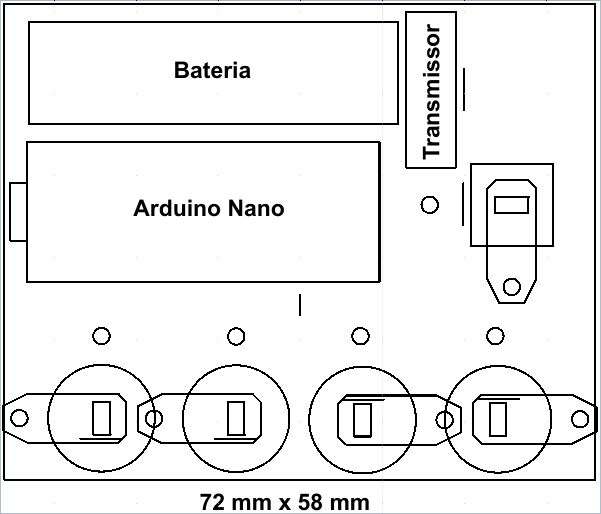
\includegraphics[scale=0.5]{figures/size-glove-module1.png}
  		\label{Fig:size-glove-module1}
		\end{figure}

		\section{Placa Embarcada}
			\subsection{Esquemático}

			Os primeiros experimentos de ligação e testes iniciais entre os componentes foram realizados ainda em protoborad. Um programa simples lia a variação de um resistor e mostrava na tela do computador. Isto foi usado para verificar como deveriam ser as conexões entre resistores, bateria, módulo transmissor e o microcontrolador Arduíno.

			O passo seguinte foi utilizar o software gratuito Kicad. Esse programa permite a inclusão de componentes e ligações na criação do esquemático do circuito. Posteriormente, possibilita a criação de uma placa de circuito impresso baseada no esquemático desenhado anteriormente. Através dele foram criados os desenhos do esquemático e da PCI do sistema eletrônico embarcado \ref{Fig:schematic-and-PCB}.

			Com o desenho da placa finalizada no Kicad, esta PCI foi impressa em papel fotográfico e o método de transferência térmica foi utilizado para fabricar uma cópia de PCI em uma placa de fenolite. Posteriormente a placa de fenolite foi corroída em uma solução de percloreto de ferro. Após a corrosão completa, a placa foi lavada e secada para finalmente ter seus pinos e componentes soldados. Chegando assim, ao resultado final \ref{Fig:phenolic-and-ready}

	\begin{figure}[!htb]
		 \centering
		 \caption{ Desenhos projetados no Kicad do (a) esquemático e (b) PCI. }
		 \subfloat[]
		 {
			 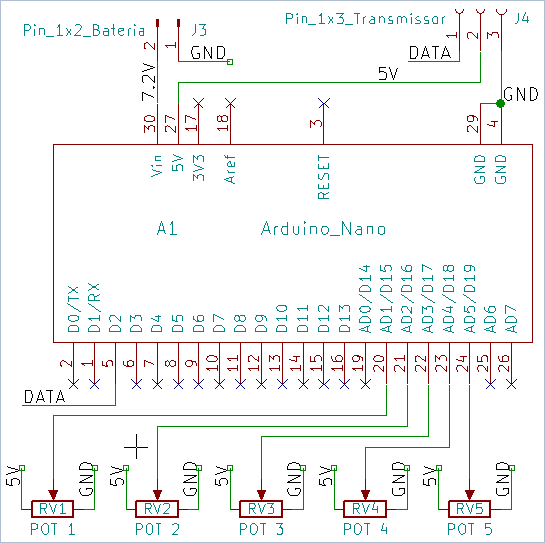
\includegraphics[width=6.5cm,keepaspectratio=true]{./figures/schematic-glove-module1.png}
		 }
		 \centering
		 \subfloat[]
		 { 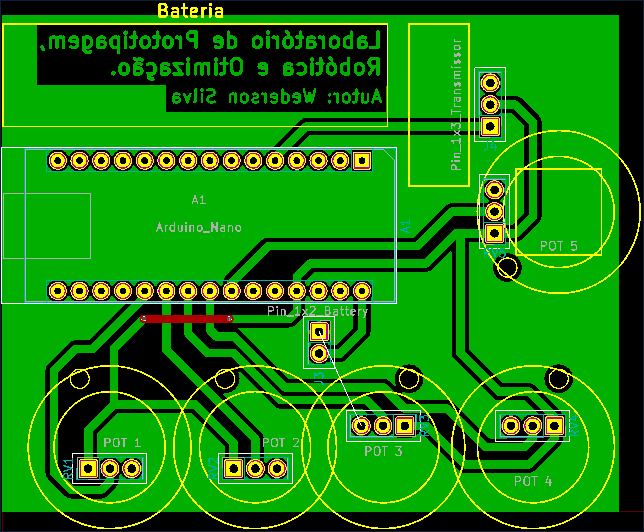
\includegraphics[width=7.5cm,keepaspectratio=true]{./figures/PCB-glove-module1.png}
		 }
		 \label{Fig:schematic-and-PCB}
		 \fonte{Produzido pelo autor}
	\end{figure}



	\begin{figure}[!htb]
		 \centering
		 \caption{ (a) Placa de fenolite após corrosão e (b) resultado final} 
		 \subfloat[]
		 {
			 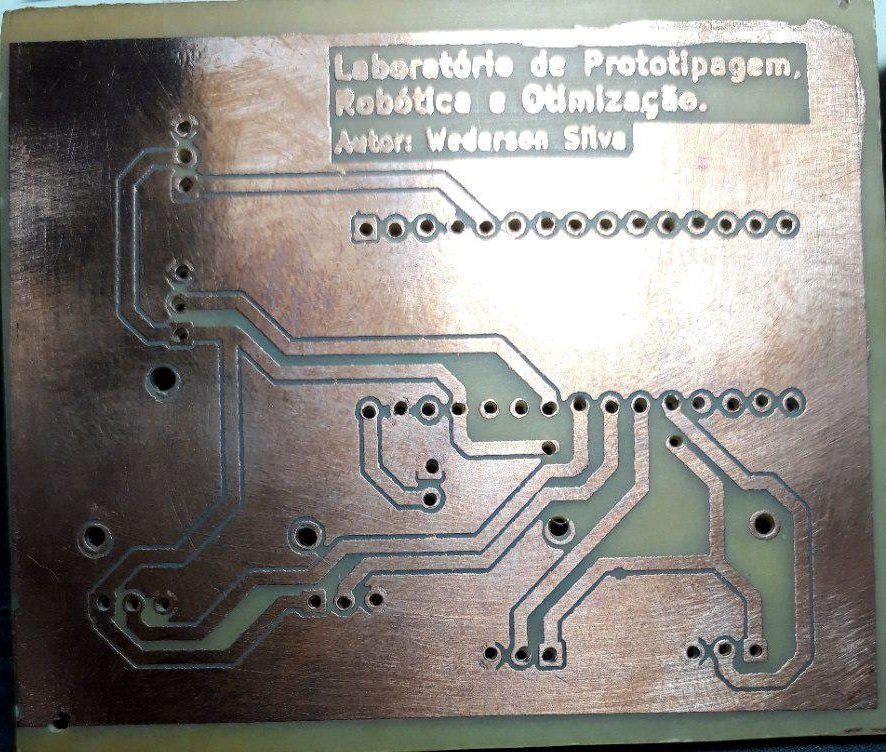
\includegraphics[width=7cm,keepaspectratio=true]{./figures/phenolic-glove-module1.jpg}
		 }
		 \centering
		 \subfloat[]
		 { 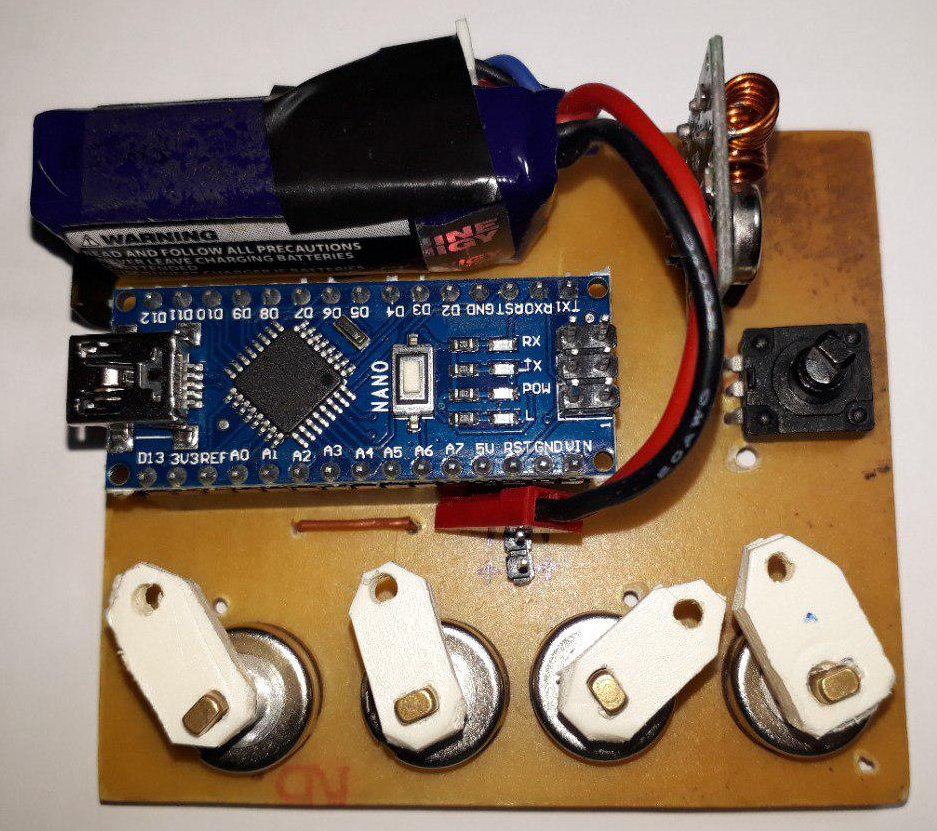
\includegraphics[width=7cm,keepaspectratio=true]{./figures/glove-module-ready1.jpg}
		 }
		 \label{Fig:phenolic-and-ready}
		 \fonte{Produzido pelo autor}
	\end{figure}


		\section{Movimento mecânico}

		\subsection{Flexão dos Dedos}

		Inspirado no movimento de flexão dos dedos da mão que é possibilitado pelos tendões, decidiu-se construir um sistema semelhante, que estaria embarcado em uma luva. O sistema deve mensurar graus de flexão e extensão dos dedos usando fios de náilon atrelados a potenciômetros que variam de acordo com a tensão e sentido do fio.

		Nesse sistema, uma das extremidades do fio de náilon é presa na ponta de um dos dedos da luva. O trajeto da extensão do fio é guiada por polias plásticas. A extremidade oposta do fio é presa ao cursor de um potenciômetro.
		Dessa forma, mantendo o fio de náilon tensionado, ao flexionar o dedo, o fio é puxado pela ponta do dedo e com isso o cursor do potênciometro é variado.
	
		A variação de resistência do potênciometro é capturada pelo microcontrolador, que traduz o movimento recebido em números que representam graus de flexão. Esses número são remapeados e transferidos ao transmissor. Este por sua vez, envia a mensagem via rádio frequência.


		\subsection{Extensão dos Dedos}

		Após a flexão dos dedos, ao realizar o movimento inverso (extenção), Nem o fio de náilon e nem o cursor do potenciômetro retornam à posição inicial. Para possibilitar que o sistema retorne à sua posição inicial, um pequeno elástico foi instalado junto ao cursor do potenciômetro. 

		Durante a flexão, o cursor gira e estica o elástico. Estando esticado, o elástico busca retomar sua posição de equilíbro realizando uma força para girar o cursor de volta à sua posição inicial. Durante o movimento de extensão do dedo, o elástico puxa o cursor do potenciômetro girando-o em sentido inverso ao que ocorreu durante a flexão. Isso ocorre enquanto o elástico estiver esticado o suficiente para exercer força sobre o cursor do potenciômetro.
		
		A força do dedo durante a flexão e a força do elástico durante a extensão giram o cursor do potenciômetro através do fio de náilon. Dessa forma, o fio e o cursor acompanham o movimento dos dedos em diferentes graus.

	\begin{figure}[!htb]
		 \centering
		 \caption{ Movimentos da luva de (a) flexão e (b) extensão} 
		 \subfloat[]
		 {
			 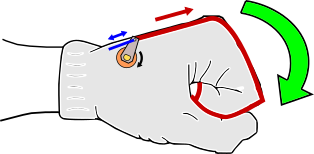
\includegraphics[width=6.5cm,keepaspectratio=true]{./figures/glove-wire-flex2.png}
		 }
		 \centering
		 \subfloat[]
		 { 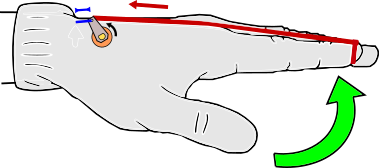
\includegraphics[width=7.5cm,keepaspectratio=true]{./figures/glove-wire-extend2.png}
		 }
		 \label{Fig:phenolic-and-ready}
		 \fonte{Produzido pelo autor}
	\end{figure}


	% ----------------------------
	%	RESULTADOS E ANÁLISES	
	% ----------------------------
	
	\chapter{Análises e Resultados}

		\section{Configurações}

		\section{Testes}

		\section{Resultados}
		

	% ----------
	%	CONCLUSÃO	
	% ----------
  \chapter{Conclusão}

		\section{Conclusões}

		\section{Trabalhos Futuros}


% ----------------------------------------------------------
% ELEMENTOS PÓS-TEXTUAIS
% ----------------------------------------------------------
\postextual
% ----------------------------------------------------------
% Referências bibliográficas
% ----------------------------------------------------------
\bibliography{referencias}

%---------------------------------------------------------------------
% INDICE REMISSIVO
%---------------------------------------------------------------------

\printindex

\end{document}
